\section{Thrust 3. Voice-Driven Features for an IDE to support VIPLs}
\label{sec:thrust3}

\begin{figure}[t]
\centering
\begin{minipage}{.48\textwidth}
%\begin{figure}[t]
\centering
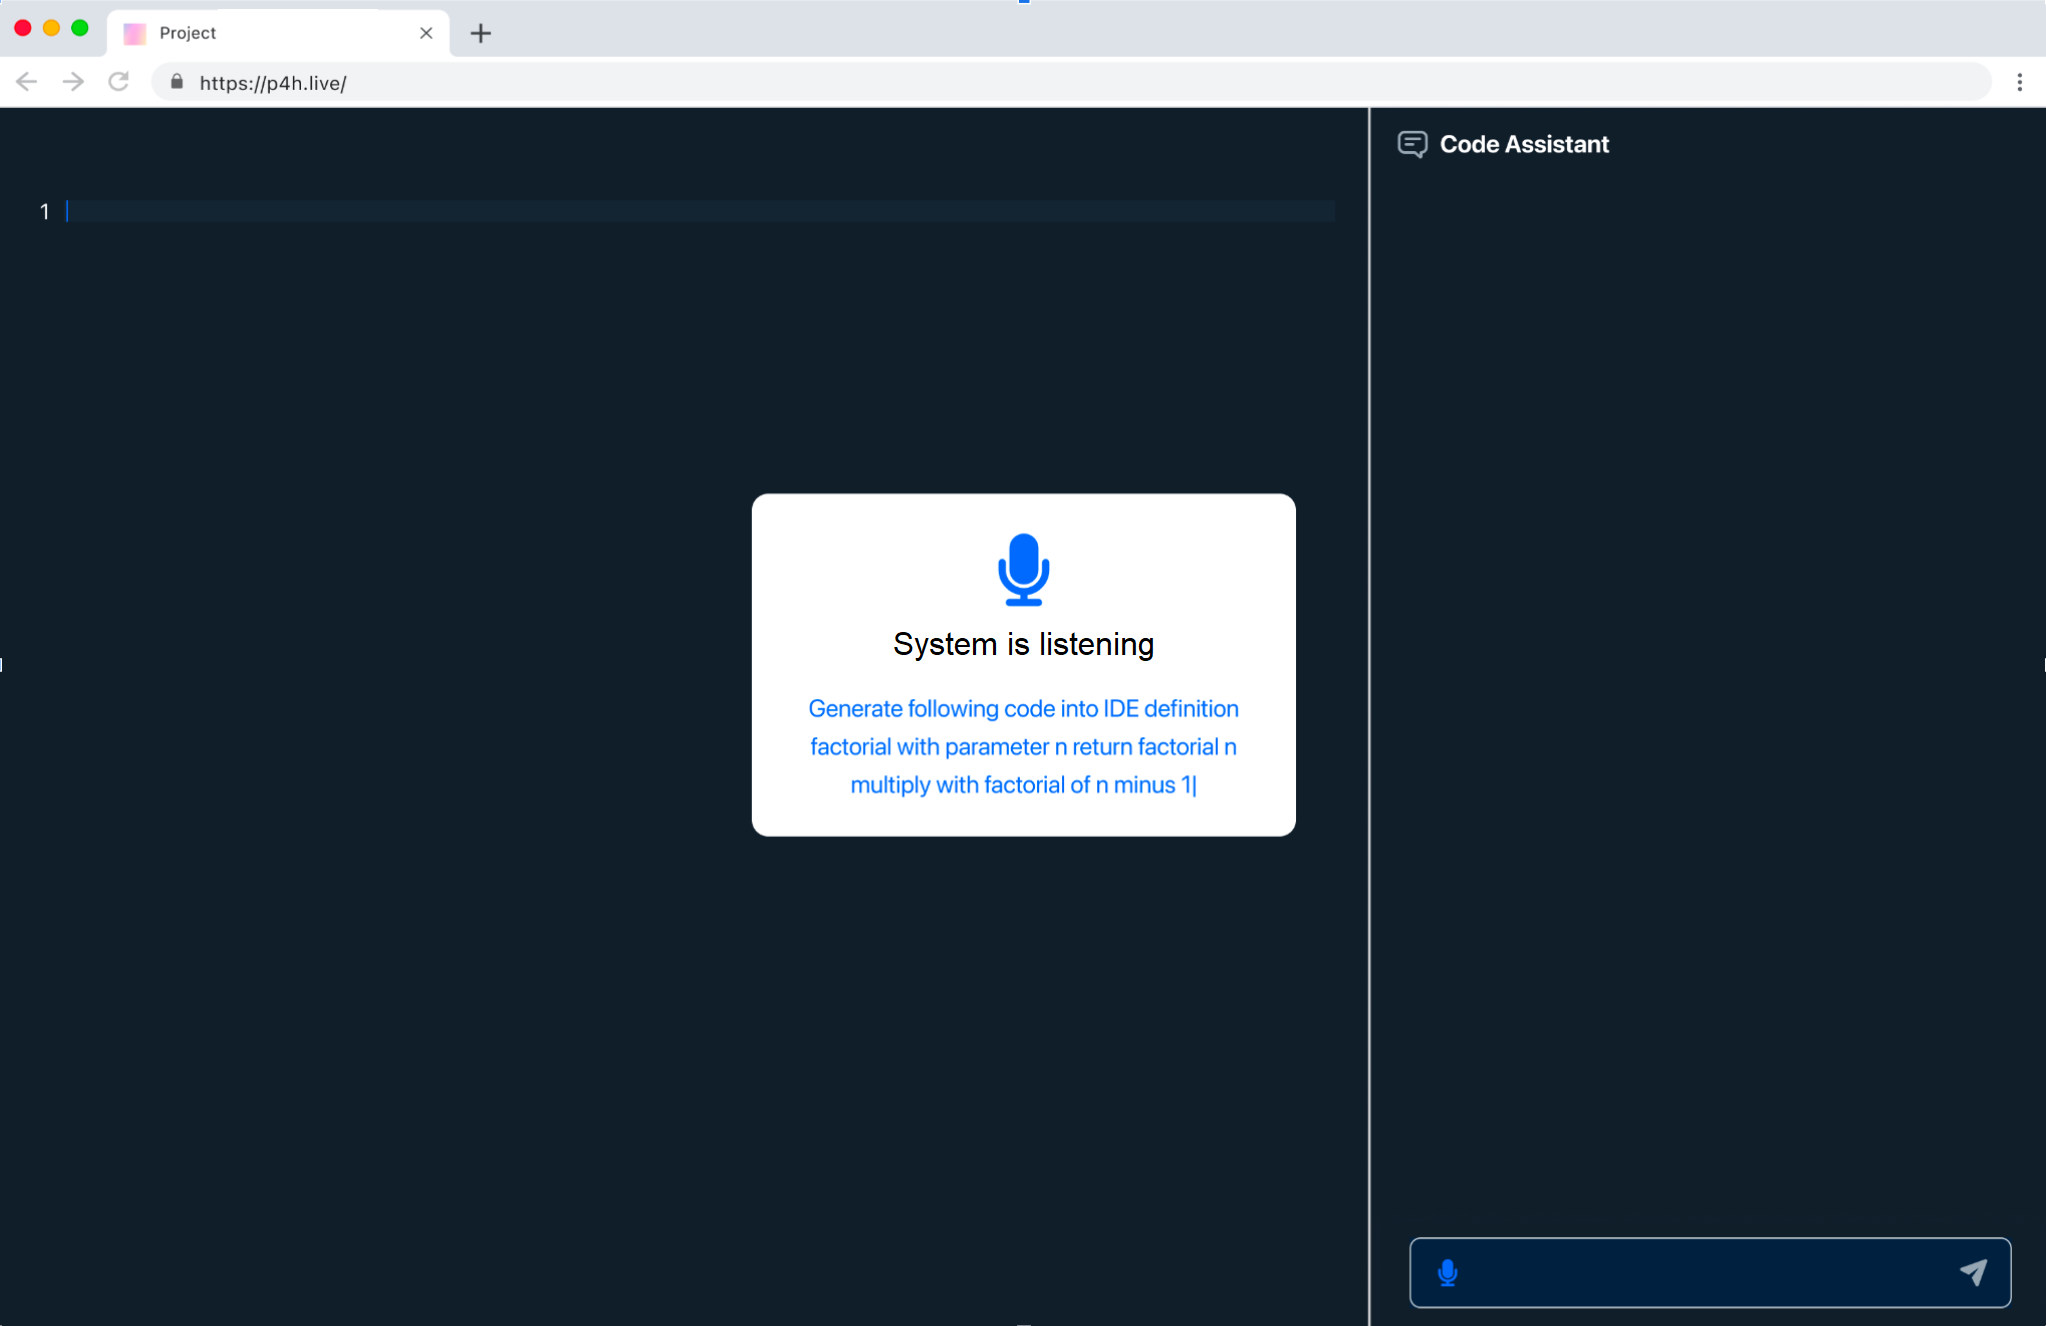
\includegraphics[width=.98\textwidth]{p4h-1}
%\caption{caption 1}
%\label{fig:left}
%\end{figure}
\end{minipage}
\begin{minipage}{.48\textwidth}
%\begin{figure}[t]
\centering
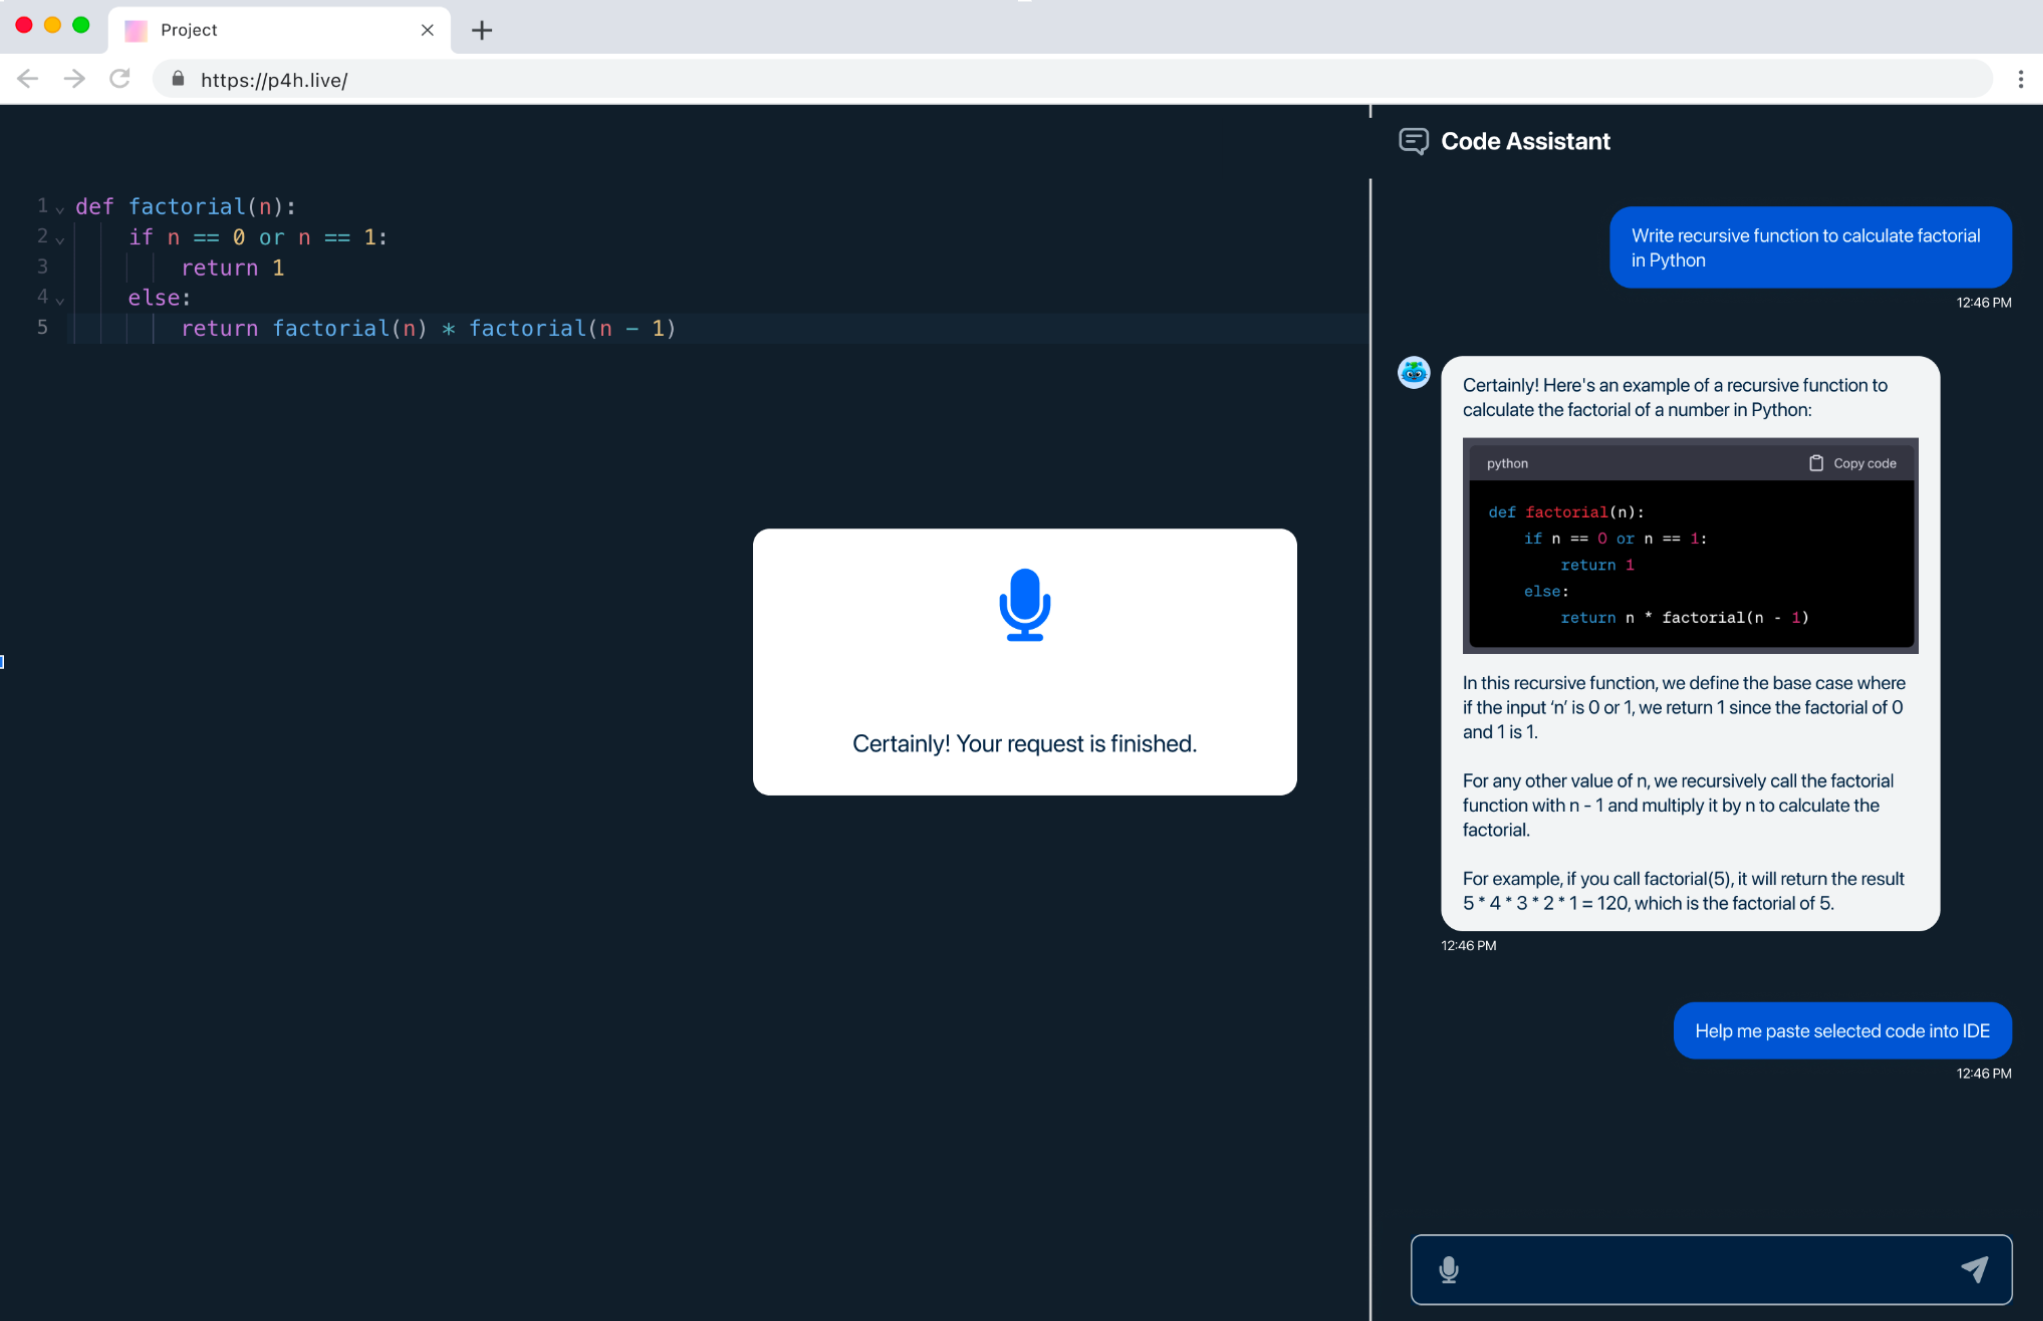
\includegraphics[width=.98\textwidth]{p4h-2}
%\caption{caption 2}
%\label{fig:right}
%\end{figure}
\end{minipage}  
\vspace{-18pt}
\caption{Caption}
\label{thrust3-one}
\end{figure}

In this use case scenario (Figure~\ref{thrust3-one}), let's explore
how a visually-impaired programmer interacts with the newly introduced
programming environment to create source code for calculating the
factorial of a number. This scenario showcases the environment's voice
interaction and code generation capabilities.

{\em Initialization}: The visually-impaired programmer initiates the
programming environment by saying, "Hey, Environment, start a new code
project for calculating factorial."

{\em Voice Interaction}: The environment responds with a synthesized voice,
"Sure, please specify the number for which you want to calculate the
factorial."

{\em User Input}: The programmer responds, "Calculate the factorial of 5."

{\em Code Generation}: The programming environment interprets the user's
request and generates the code snippet using advanced voice
recognition and generative AI technologies.  The environment then
communicates, "I've generated the code to calculate the factorial of
5. Here's the code for you:".

{\em Verification}: The generated code is read back to the user through synthesized speech, and the user can confirm its accuracy.
The user says, "Please read back the generated code."

{\em Confirmation}: The environment reads the code aloud, "Def factorial(n): If n equals 0, return 1. Else, return n times factorial(n minus 1). Result equals factorial(5). Print 'The factorial of 5 is:' and the result." The user confirms that the code accurately reflects their intent.

{\em Execution}: The programmer can proceed to execute the code by saying, "Execute the code." The environment executes the code, and the synthesized speech reads the result, "The factorial of 5 is: 120."

{\em Documentation}: The programmer can further enhance the code by documenting it using voice commands. For example, they can say, "Add a comment: This code calculates the factorial of a number."

{\em Integration}: If the programmer has an existing project, they can
integrate this code seamlessly into their project using voice
commands, ensuring a cohesive workflow.
